%%%%%%%%%%%%%%%%%%%%%%%%%%%%%%%%%%%%%%%%%%%%%%%%%%%%%%%%%%%%%%%%%%%%%%%%%%%%%%%%
%              Capitulo 4: Arquitectura general del sistema                    %
%%%%%%%%%%%%%%%%%%%%%%%%%%%%%%%%%%%%%%%%%%%%%%%%%%%%%%%%%%%%%%%%%%%%%%%%%%%%%%%%

\chapter{Arquitectura general del sistema}

El sistema está estructurado en una serie de módulos lógicos que representan una
tarea de alto nivel. Un módulo lógico se compone a su vez de diversos módulos
funcionales o procesos, los cuáles llevan a cabo una tarea concreta y se comunican con
otros módulos funcionales del mismo módulo lógico para llevar a cabo dicha tarea de alto
nivel.

La tarea que un módulo funcional lleva a cabo puede realizarse de forma automática o
puede llegar a requerir de la interacción con el usuario para poder ser completada.
Cabe destacar además que, en determinados casos, los módulos funcionales de un módulo
lógico pueden comunicarse con los módulos funcionales de otros módulos lógicos, lo cuál se
describirá más detenidamente más adelante.

Por lo pronto, los módulos lógicos principales que se han considerado a la hora de definir
la arquitectura son los siguientes:

\begin{itemize}[label=\textbullet]
    \item Un módulo de interacción con el usuario (\textit{User interaction}).
    \item Un módulo de planificación (\textit{Planning}).
    \item Un módulo de monitorización y ejecución del plan (\textit{Plan Execution \& Monitoring}).
\end{itemize}

En la figura \ref{fig:system_arch} pueden verse los distintos módulos lógicos y funcionales que
componen el sistema, además de cómo están organizados, cómo se comunican y qué información se
envían entre ellos.

\begin{figure}[H]
    \centering
    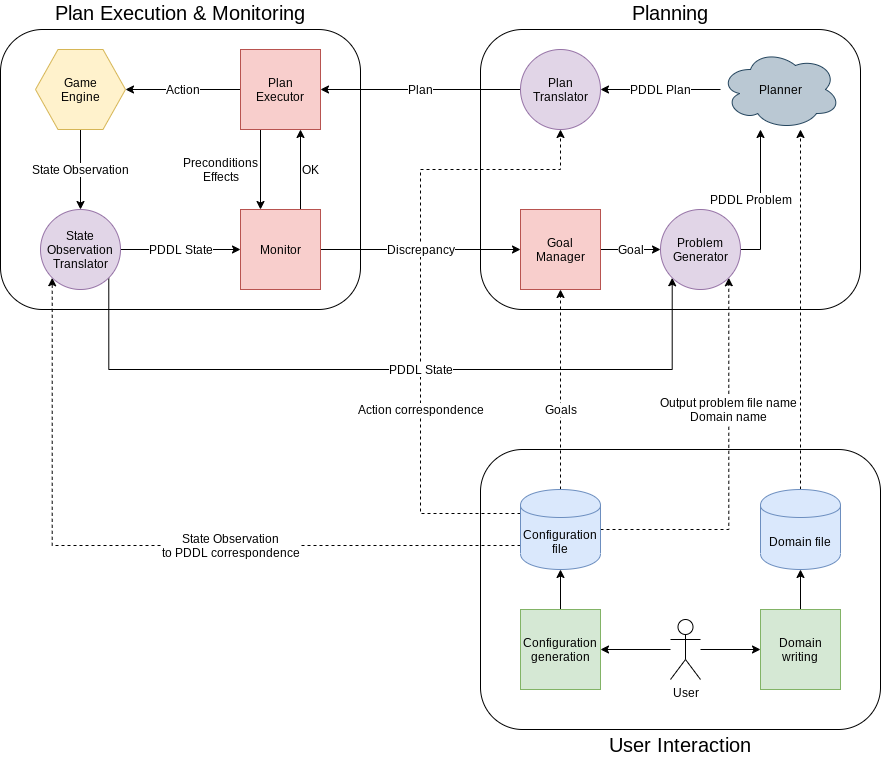
\includegraphics[scale=0.4]{img/CH04/system_arch.png}
    \caption{Esquema de la arquitectura general del sistema.}
    \label{fig:system_arch}
\end{figure}

Tomando en consideración dicho esquema, vamos a comentar brevemente cuál es
la funcionalidad básica de cada módulo lógico y cómo interactúan entre ellos.
En el próximo capítulo desglosaremos cada uno de ellos y estudiaremos los módulos
funcionales que los componen, de forma que se obtendrá una mejor visión de cómo
funciona cada componente y de cómo interactúa con las demás.

Empecemos por la parte fundamental, la cuál es el \textbf{módulo de interacción con el usuario}.
Como se puede suponer y por lo que se ha comentado anteriormente, este es el módulo
menos automatizado, ya que es con el que interactúa directamente el usuario. Es aquí
donde se encuentran dos de los procesos más importantes: la creación del dominio
(\textit{Domain Writing}) y la creación del archivo de configuración
(\textit{Configuration Generation}) que utilizará el sistema.

Por una parte, el usuario tiene que definir el dominio de planificación, que es el que se
utilizará en el sistema para representar el estado del juego en formato \texttt{PDDL}.
Por otra parte, el usuario debe especificar una serie de parámetros en el archivo de
configuración, los cuáles se utilizarán en el sistema para, entre otras cosas, traducir los
estados de observación del juego a predicados \texttt{PDDL}.

El siguiente módulo lógico que vamos a comentar es el \textbf{módulo de planificación}.
Este módulo se encarga de gestionar los objetivos cuando sea necesario, estableciendo el
objetivo actual y determinando cuáles se han cumplido y cuáles no. También es el responsable
de obtener un plan válido hasta un predicado objetivo dado, y de traducir posteriormente
dicho plan para que pueda ser ejecutado en el entorno de juego.

Por último tenemos el \textbf{módulo de ejecución del plan y de monitorización}. Como su
propio nombre indica, este módulo se encarga de ejecutar el plan obtenido por el módulo
de planificación y de monitorizar dicha ejecución, determinando en el proceso si se ha
producido alguna discrepancia, y si por tanto hace falta replanificar. En el proceso
tiene que realizar la traducción del estado de observación del juego a predicados
\texttt{PDDL}, ya que esta información se utiliza por el monitor para estudiar la
existencia de discrepancias.

En cuanto a las interacciones entre los módulos, el módulo de ejecución del plan y de
monitorización y el de planificación interactúan directamente entre ellos. El primero
comunica al segundo si se ha producido alguna discrepancia, y el segundo debe determinar
un nuevo objetivo y encontrar un plan hasta dicho objetivo. Posteriormente, el plan obtenido
es comunicado al primer módulo, el cuál se encargará de hacer las operaciones pertinentes
con él.

El módulo de interacción con el usuario se comporta como un proveedor con los otros dos
módulos, ya que les proporciona la información necesaria para que éstos puedan
llevar a cabo ciertas tareas. Al funcionar como un proveedor, la comunicación es unilateral,
ya que no obtiene ningún tipo de respuesta de ellos.
